\documentclass{beamer}
\usepackage[utf8]{inputenc}
\usetheme{Madrid}
\usecolortheme{default}
\usepackage{amsmath,amssymb,amsfonts,amsthm}
\usepackage{txfonts}
\usepackage{tkz-euclide}
\usepackage{listings}
\usepackage{adjustbox}
\usepackage{array}
\usepackage{tabularx}
\usepackage{gvv}
\usepackage{lmodern}
\usepackage{circuitikz}
\usepackage{tikz}
\usepackage{graphicx}

\setbeamertemplate{page number in head/foot}[totalframenumber]

\usepackage{tcolorbox}
\tcbuselibrary{minted,breakable,xparse,skins}



\definecolor{bg}{gray}{0.95}
\DeclareTCBListing{mintedbox}{O{}m!O{}}{%
  breakable=true,
  listing engine=minted,
  listing only,
  minted language=#2,
  minted style=default,
  minted options={%
    linenos,
    gobble=0,
    breaklines=true,
    breakafter=,,
    fontsize=\small,
    numbersep=8pt,
    #1},
  boxsep=0pt,
  left skip=0pt,
  right skip=0pt,
  left=25pt,
  right=0pt,
  top=3pt,
  bottom=3pt,
  arc=5pt,
  leftrule=0pt,
  rightrule=0pt,
  bottomrule=2pt,
  toprule=2pt,
  colback=bg,
  colframe=orange!70,
  enhanced,
  overlay={%
    \begin{tcbclipinterior}
    \fill[orange!20!white] (frame.south west) rectangle ([xshift=20pt]frame.north west);
    \end{tcbclipinterior}},
  #3,
}
\lstset{
    language=C,
    basicstyle=\ttfamily\small,
    keywordstyle=\color{blue},
    stringstyle=\color{orange},
    commentstyle=\color{green!60!black},
    numbers=left,
    numberstyle=\tiny\color{gray},
    breaklines=true,
    showstringspaces=false,
}


\title 
{2.2.21}
\date{August 31,2025}


\author 
{Manohar-AI25BTECH11028}



\begin{document}


\frame{\titlepage}
\begin{frame}{Question}
If the angle between two lines is $\pi/4$ and slope of one of the lines is $1/2$,find the slope of the other line.
\end{frame}





\begin{frame}{Equation}
From the given Information,

Angle between the lines is $\pi/4$

The angle $\theta$ between $\vec{a},\vec{b}$, is given by 

\begin{align}
\cos \theta = \frac{\vec{a}^\top \vec{b}}{\|\vec{a}\| \|\vec{b}\|}
\end{align}
\end{frame}
\begin{frame}{Solution}

let vector $\vec{A}$ be the line slope 1/2  and $\vec{B}$ be the line with slope $m_2$

\begin{align}
    \vec{A}=\myvec{1\\ 1/2} \\
    \vec{B}=\myvec{1\\m_2}
\end{align}

\begin{align}
    \cos{\pi/4} = \frac{\vec{A}^\top \vec{B}}{\|\vec{A}\| \|\vec{B}\|}
\end{align}


\end{frame}

\begin{frame}{Solution}
Now,
\begin{align}
       \vec{A}^\top \vec{B}&=\myvec{1\\1/2}^\top \myvec{1\\m_2}=1^2+m_2/2\\
\|\vec{A}\| &= \sqrt{1^2 + \left(\frac{1}{2}\right)^2} = \sqrt{1 + \frac{1}{4}} = \sqrt{\frac{5}{4}} = \frac{\sqrt{5}}{2} \\
\|\vec{B}\| &= \sqrt{1^2 + m_2^2} = \sqrt{1 + m_2^2}
\end{align}

From this,

\begin{align}
    \frac{1}{\sqrt{2}}*\frac{\sqrt{5}}{2}*\sqrt{1+m_2^2}=1+\frac{m_2}{2}\\
    \sqrt{5}*\sqrt{1+m_2^2}=\sqrt{2}(2+m_2)
\end{align}
 

\end{frame}

\begin{frame}{Solution}

Now squaring on both sides;
\begin{align}
    5+5m_2^2=2(4+m_2^2+4m_2)\\
    3m_2^2-8m_2-3=0
\end{align}

Therefore,
\begin{align}
    m_2=3or-1/3
\end{align}    
\end{frame}


\begin{frame}[fragile]
    \frametitle{C Code}

    \begin{lstlisting}

#include <stdio.h>
#include <math.h>

// Function to find slopes of second line given m1 and angle
int find_other_slopes(double m1, double theta, double *slopes) {
    // Equation derived: tan(theta) = |(m2 - m1) / (1 + m1*m2)|
    // Rearranged: (m2 - m1) = +/- tan(theta) * (1 + m1*m2)

    double t = tan(theta);
    

    \end{lstlisting}
\end{frame}

\begin{frame}[fragile]
    \frametitle{C Code}
    \begin{lstlisting}
    
        // Case 1: (m2 - m1) = +t(1 + m1*m2)
    // => m2 - t*m1*m2 = m1 + t
    // => m2(1 - t*m1) = m1 + t
    slopes[0] = (m1 + t) / (1 - t*m1);

    // Case 2: (m2 - m1) = -t(1 + m1*m2)
    // => m2 + t*m1*m2 = m1 - t
    // => m2(1 + t*m1) = m1 - t
    slopes[1] = (m1 - t) / (1 + t*m1);

    return 2;  // number of solutions
    }

    \end{lstlisting}
\end{frame}

\begin{frame}[fragile]
    \frametitle{Python+C Code}
    \begin{lstlisting}
    
  import ctypes
import numpy as np
import matplotlib.pyplot as plt

# Load shared library
lib = ctypes.CDLL("./libline_angle.so")

# Define function signature
lib.find_other_slopes.argtypes = [ctypes.c_double, ctypes.c_double, ctypes.POINTER(ctypes.c_double)]
lib.find_other_slopes.restype = ctypes.c_int





    \end{lstlisting}
\end{frame}

\begin{frame}[fragile]
    \frametitle{Python+C Code}
    \begin{lstlisting}
 def other_slopes_c(m1, theta):
    result = (ctypes.c_double * 2)()
    n = lib.find_other_slopes(m1, theta, result)
    return [result[i] for i in range(n)]

m1 = 0.5
theta = np.pi/4

slopes = other_slopes_c(m1, theta)
print("Slopes from C library:", slopes)



    \end{lstlisting}
\end{frame}

\begin{frame}[fragile]
    \frametitle{Python+C Code}
    \begin{lstlisting}
# --- Plotting ---
x = np.linspace(-10, 10, 100)

plt.axhline(0, color='k')
plt.axvline(0, color='k')

plt.plot(x, m1*x, 'r', label=f"Slope m1={m1}")
plt.plot(x, slopes[0]*x, 'g', label=f"Slope m2={slopes[0]:.2f}")
plt.plot(x, slopes[1]*x, 'b', label=f"Slope m2={slopes[1]:.2f}")

plt.legend()
plt.grid(True)
plt.xlabel("x")
plt.ylabel("y")
plt.title("Lines with given angle")


    \end{lstlisting}
\end{frame}


\begin{frame}[fragile]
    \frametitle{Python+C Code}
    \begin{lstlisting}


# Save before show
plt.savefig("/storage/emulated/0/matrix/Matgeo/2.2.21/figs/Figure_1.png", dpi=300, bbox_inches='tight')
plt.show()
    \end{lstlisting}
\end{frame}


\begin{frame}{Plot}
    \centering
    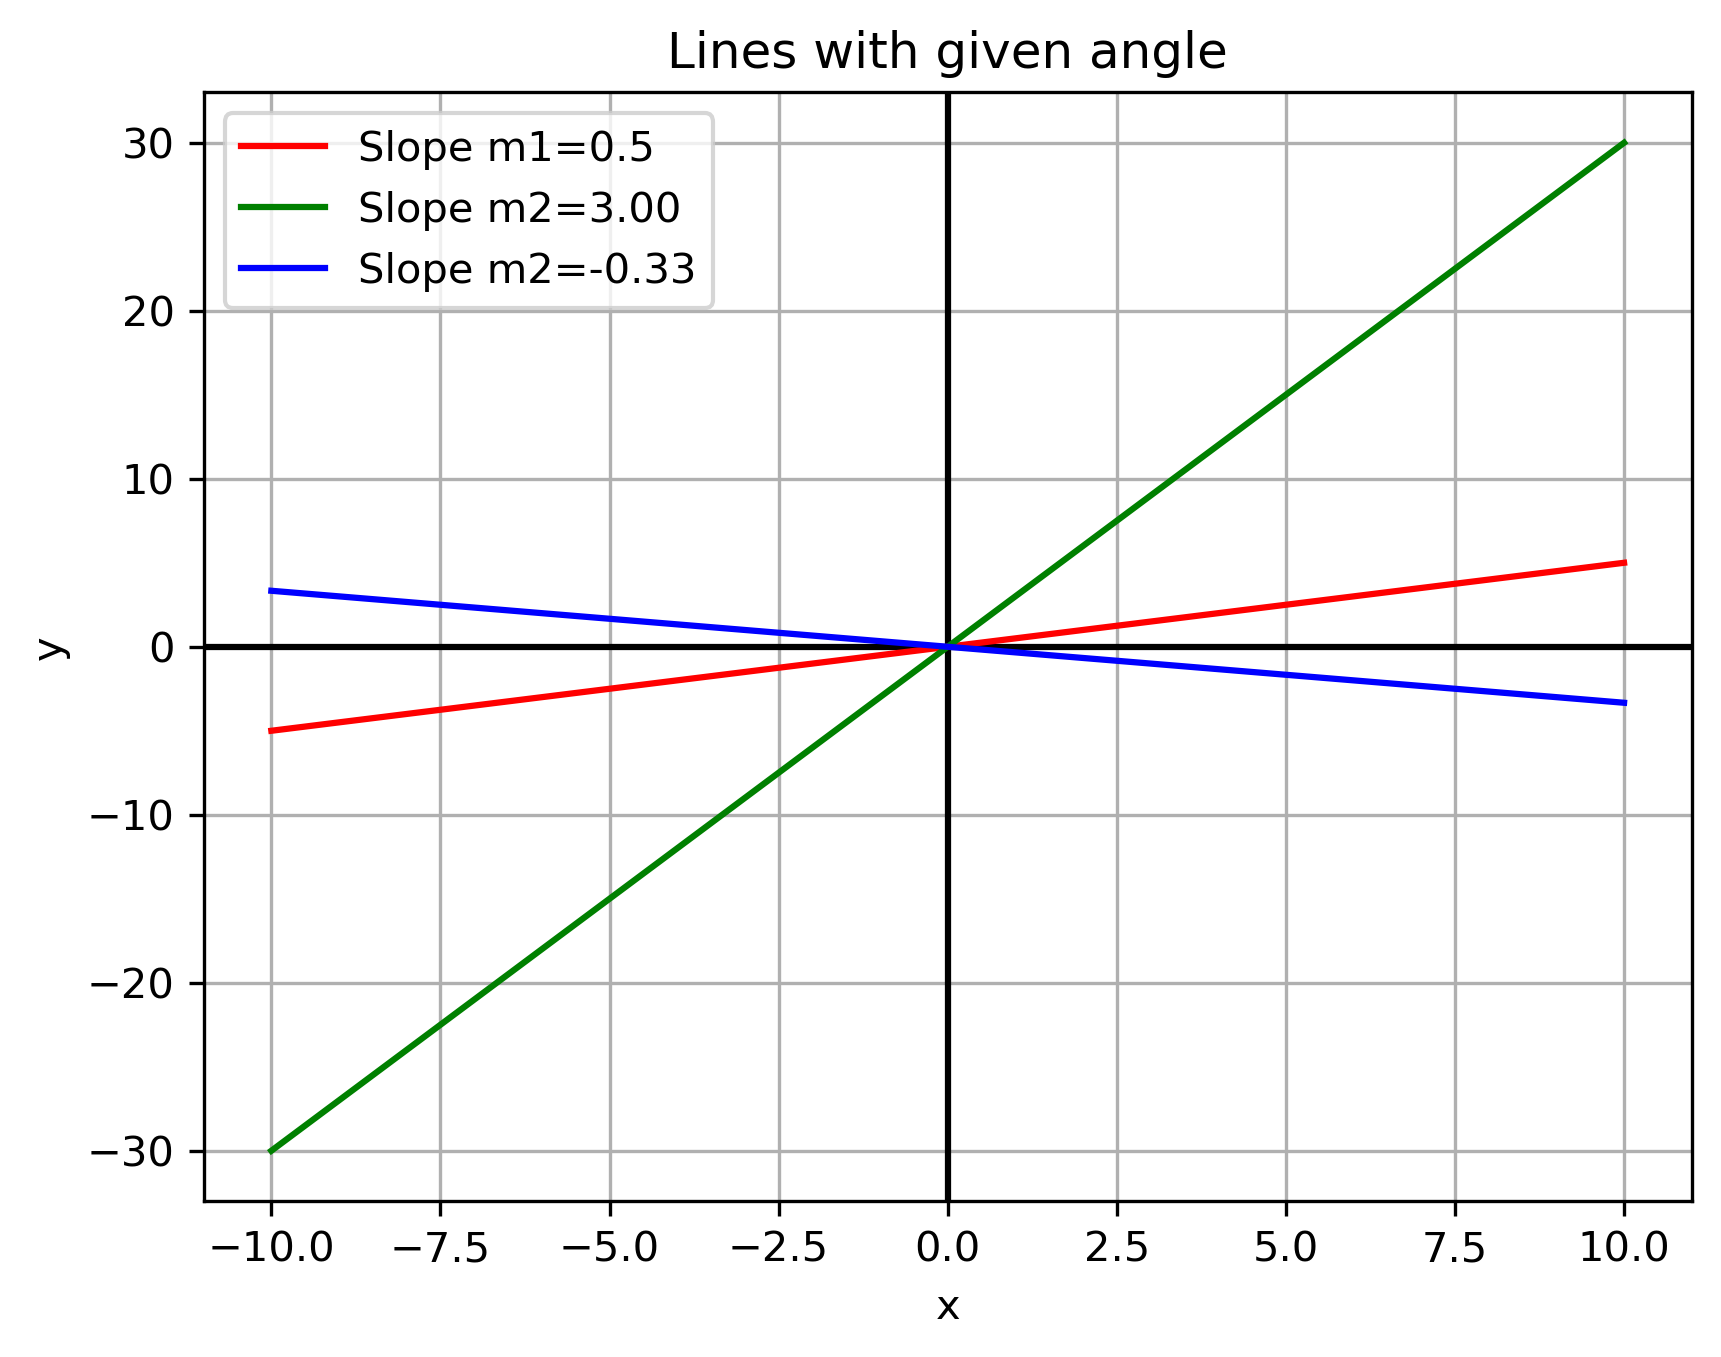
\includegraphics[width=\columnwidth, height=0.8\textheight, keepaspectratio]{figs/figure_1.png}     
\end{frame}

\begin{frame}[fragile]
    \frametitle{Python Code}
    \begin{lstlisting}
        import numpy as np

def other_slopes(m1, theta):
    t = np.tan(theta)
    m2_1 = (m1 + t) / (1 - t*m1)
    m2_2 = (m1 - t) / (1 + t*m1)
    return m2_1, m2_2

m1 = 0.5
theta = np.pi/4

slopes = other_slopes(m1, theta)
print("Slopes of other line(s):", slopes)



    \end{lstlisting}
\end{frame}

\begin{frame}[fragile]
    \frametitle{Python Code}
    \begin{lstlisting}
    # --- Plotting ---
import matplotlib.pyplot as plt

x = np.linspace(-10, 10, 100)

plt.axhline(0, color='k')
plt.axvline(0, color='k')

plt.plot(x, m1*x, 'r', label=f"Slope m1={m1}")
plt.plot(x, slopes[0]*x, 'g', label=f"Slope m2={slopes[0]:.2f}")
plt.plot(x, slopes[1]*x, 'b', label=f"Slope m2={slopes[1]:.2f}")

plt.legend()
plt.grid(True)
plt.xlabel("x")
plt.ylabel("y")
plt.title("Lines with given angle")
    \end{lstlisting}
\end{frame}

\begin{frame}[fragile]
    \frametitle{Python Code}
    \begin{lstlisting}
     # Save before show
plt.savefig("/storage/emulated/0/matrix/Matgeo/2.2.21/figs/Figure_1.png", dpi=300, bbox_inches='tight')
plt.show()   
    \end{lstlisting}
    
\end{frame}
\end{document}
